\documentclass[8pt]{extarticle} 
\usepackage{graphicx} % Required for inserting images
\usepackage{amsfonts}
\usepackage{enumitem}
\usepackage[hidelinks]{hyperref}
\usepackage{graphicx}
\usepackage{textcomp}
\usepackage{amsmath}
\usepackage{multicol}
\usepackage{mathabx}
\usepackage[bottom=0.5cm, right=1.5cm, left=1.5cm, top=1.5cm, headheight=16pt]{geometry}
\usepackage{amssymb}
\usepackage{amsthm}
\usepackage{amsmath}
\usepackage{physics}
\usepackage{cancel}
\usepackage{mathtools}
\usepackage{array}
\usepackage{tikz}
\def\checkmark{\tikz\fill[scale=0.4](0,.35) -- (.25,0) -- (1,.7) -- (.25,.15) -- cycle;} 
\makeatletter
\newcases{crcases}{\quad}{%
  \hfil$\m@th\displaystyle{##}$\hfil}{\hfil$\m@th\displaystyle{##}$}{\lbrace}{.}
\makeatother
\usepackage{mdframed}
\usepackage{tikzlings}
\usepackage{tikzducks}
\usepackage{animate}



\title{\textbf{Fundamental Theorem of Calculus}}
\author{\textbf{Connor Li}}
\date{\textbf{March 2024}}

\newmdenv{boxedsection}

\begin{document}

\maketitle


\section*{Contact Information}
\begin{itemize}
    \item \underline{Author}: Connor Li
    \item \underline{Email}: connor.li@columbia.edu
    \item \underline{Phone Number}: (404) 642-6292
    \item \underline{LinkedIn}: \href{https://www.linkedin.com/in/connor-li-4871a71a9/}{Click Here}
    \item \underline{Personal Website}: \href{https://connorli18.github.io/}{Click Here}
    \item \underline{GitHub}: \href{https://github.com/connorli18}{Click Here}
    \item \underline{Resume}: \href{https://drive.google.com/file/d/1G4QryPZy70d9OCKWtcJPA6su5gIfjmIe/view?usp=sharing}{Click Here}
\end{itemize}
\vspace{2cm}
\tableofcontents

\pagebreak
\section{Overview}
\subsection{The Goal}
The goal of this document is to provide a comprehensive overview of the Fundamental Theorem of Calculus from both an analytical and practical standpoint. The content of the document will hopefully tie together important proofs, concepts, and give you a nice reminder/refresher over one of the most important concepts ever introduced in higher-level mathematics.
\subsection{Top Level Note}
The Fundamental Theorem of Calculus is a cornerstone in mathematics, linking two principal concepts: differentiation and integration. It highlights that differentiation and integration are inverse processes of each other. This theorem underpins the ability to compute the area under a curve using antiderivatives, illustrating a deep and intrinsic connection between rates of change (differential calculus) and accumulation of quantities (integral calculus). Essentially, it provides a comprehensive framework that allows for the practical application of calculus in solving real-world problems, by demonstrating how these seemingly disparate concepts are fundamentally intertwined.
\section{Establishing a Basis}
\subsection{The Derivative}
\subsubsection{Introduction}
If you've taken any math class, you're probably familiar with the concept of slope. Whether you've been taught it as ``rise over run'' or ``change in $y$ over change in $x$'', the concept is the same for lines. Intuitively, it tells you how fast a line is changing at a given point. But, not every interesting graph is a line, and oftentimes the graphs that we are interested in do not have constant slope. Take this function, for example.
\vspace{0.5cm}
$$
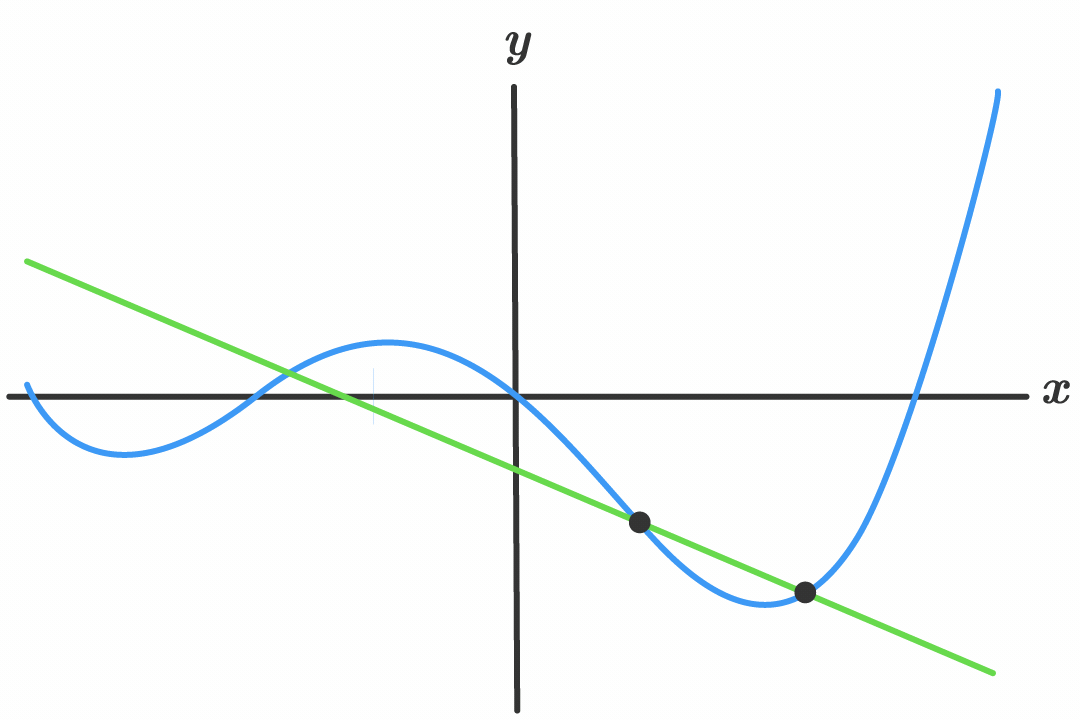
\includegraphics[width=6cm]{images/slope-0.png} \quad \quad \quad \quad 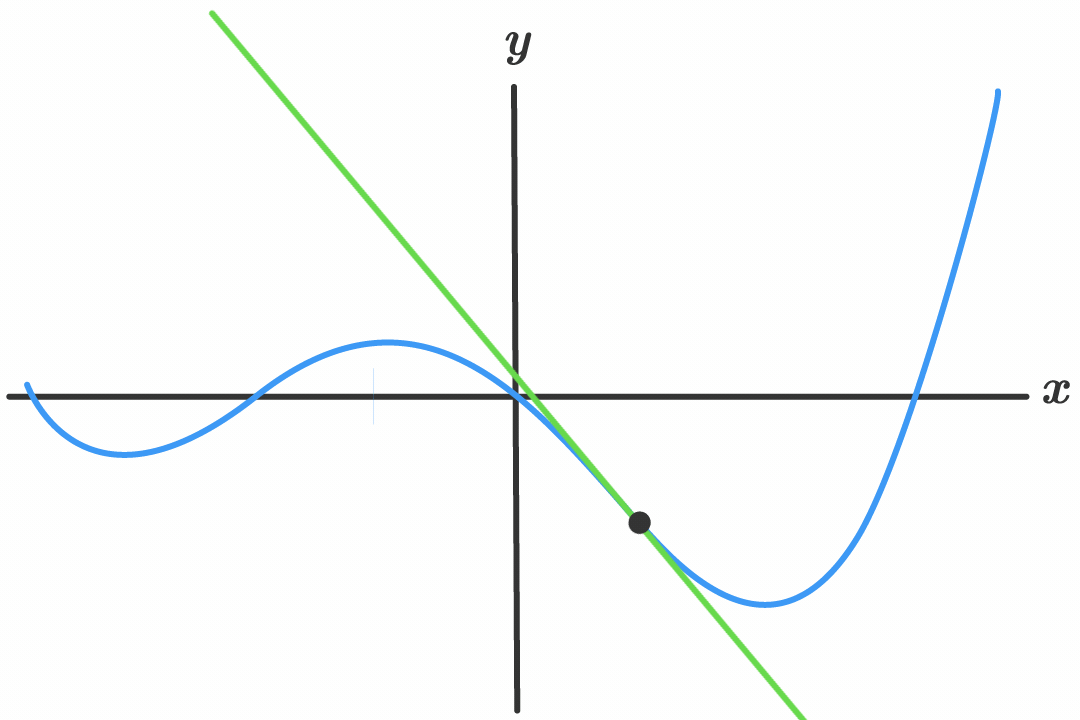
\includegraphics[width=6cm]{images/slope-132.png}
$$
As you can clearly see, at every point, the slope of the function is changing. So, we formalize our definition of the derivative as the instantaneous rate of change of a function at a given point. Basically, if you take tangent lines (lines that touch the graph at only one point) at every point on the graph, the slope of those lines is the derivative at the respective point.
\subsubsection{The Definition}
Using the intuition provided above, we can formally define the derivative of a function at any given point. Essentially, we can pick any two points of the function and take the slope of the line connecting them. And, as we decrease the distance that separates the two points, the slope of the line connecting them will approach the slope of the tangent line at the point. So, we present the following definition.
\begin{boxedsection}
\textbf{Definition (Derivative at a Point)}: Let $f(x)$ be any function. Then, we can say the derivative of $f(x)$ at any point $a$ (if it exists), which we will denote $f'(a)$, is defined by
$$
f'(a) = \lim_{x \rightarrow a} \frac{f(x) - f(a)}{x-a} = \lim_{h \rightarrow 0} \frac{f(a+h) - f(a)}{h}
$$
\underline{Note}: These definitions are the same under the change of variables $h = x -a$. 
\end{boxedsection}
If $f'(a)$ exists and is well defined at every point in the function's domain, then we can say that there exists some function $f'(x)$ that represents the derivative at every point. This is the case for most functions that we encounter in practice, and we call this function $f'(x)$ the derivative of $f(x)$.
\begin{boxedsection}
\textbf{Definition (Derivative of a Function):} A function $f(x)$ is called differentiable at $x=a$ if $f'(a)$ exists and is called differentiable on an interval if it is differentiable at every point in the interval. The function $f'(x)$ is called the derivative of $f(x)$.
\end{boxedsection}
\subsection{The Integral}
\subsubsection{Introduction}
The integral is a concept related to find ``the area under the curve''. Very generally, the concept relies on taking ``boxes'' of some width where the height of the boxes are defined by the function $f(x)$. If you add these boxes together, you get an approximation of the area under the curve.
$$
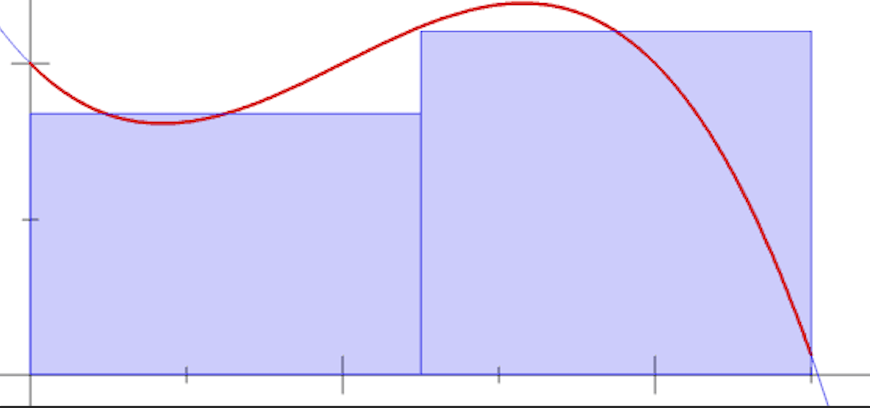
\includegraphics[width=7cm]{images/part1integral.png} \quad \quad \quad \quad
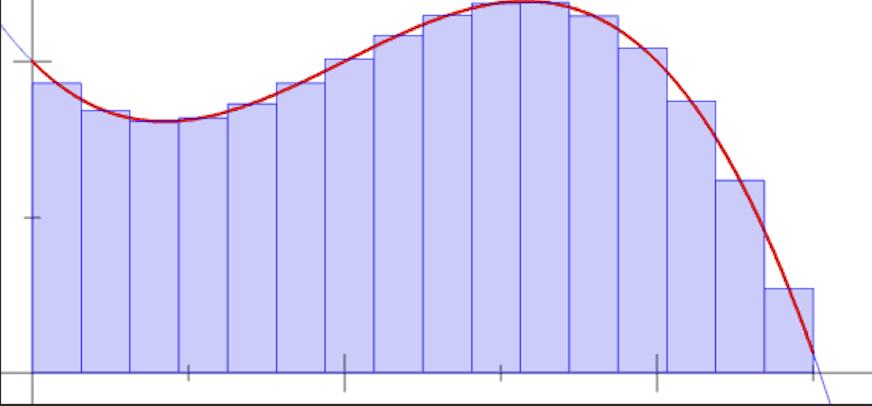
\includegraphics[width=7cm]{images/part2integral.png}
$$
The method of taking these boxes is demonstrated in the pictures above. If you notice, the approximation gets better as the width of the boxes decreases. This is because the approximation gets closer to the actual area under the curve. So, we can formally define the integral as the limit of these approximations.
\subsubsection{The Definition}
The definite integral from $a$ to $b$ of a function $f(x)$ is ``the area under the curve'' of $f(x)$ from point $a$ to point $b$, which we denote as follows.
$$
\int_a^b f(x) \;dx
$$
In this case, the $dx$ is what we call the ``term of integration,'' which is a notation that tells us that we are integrating with respect to $x$ (i.e. finding the area with respect to a change in $x$). Using the intuition above, we can define the definite integral as follows.
\begin{boxedsection}
  \textbf{Definition (Definite Integral):} Let $f(x)$ be any function over the interval $x \in [a,b]$. If we divide $[a,b]$ into $n$ subintervals of equal width $(\Delta x)$, and pick any point over each divided interval $x_i^*$, then the definition integral is defined as follows.
  $$
  \int_a^b f(x) \;dx = \lim_{n\rightarrow\infty} \sum_{i=1}^n f(x_i^*) \Delta x 
  $$
  \underline{Note}: In this case, we are taking $n$ of these small intervals where the width of the mini-rectangle is $\Delta x$ and the height of said rectangle is $f(x_i^*)$. Since we take $n \rightarrow \infty$, we are adding up more and more rectangles to get a better (almost perfect) approximation of the area under the curve.
\end{boxedsection}
Now, you're probably wondering about indefinite integrals. Like derivatives, we are interested in the expression $\int f(x)\;dx$ without bounds. Specifically, we want to know if it's possible to express the indefinite integral as a function of $x$. To answer this question, we must use the Fundamental Theorem of Calculus, which we will discuss in the next section.
\section{Precursors to the Theorem}
\subsection{Overview}
To rigorously prove the Fundamental Theorem of Calculus and elucidate the deep-seated connection between the operations of integration and differentiation, it is imperative to invoke a suite of fundamental theorems. This methodology serves not only to validate the theorem itself but also to illuminate the inherent linkage between integration and differentiation, thereby providing a solid foundation for a substantial portion of calculus theory. The subsequent discussion will employ analytical techniques useful in any higher-level proofs course.
\subsection{Extreme Value Theorem}
The Extreme Value Theorem is a fundamental theorem in calculus that we will use to prove the Fundamental Theorem of Calculus.
Intuitively, the theorem is quite simple. It states that if a function is continuous on a closed interval $[a,b]$, then the function must attain some maximum and minimum value over the interval $[a,b]$.
\begin{boxedsection}
  \textbf{Theorem:} If $f$ is continuous function over the closed, bounded interval of $[a,b]$, then $f$ attains some maximum and minimum value over the interval $[a.b]$.\\
  \\
  \textbf{Proof:} The proof is quite complex, but a version of it is linked \href{https://mathcenter.oxford.emory.edu/site/math111/proofs/extremeValueTheorem/}{here}.
\end{boxedsection}
\subsection{Mean Value Theorem}

\section{The Fundamental Theorem of Calculus}
\subsection{Part 1}
\subsection{Part 2}
\subsection{Part 3}

\section{Conclusion}



https://mathworld.wolfram.com/FundamentalTheoremsofCalculus.html


\end{document}
